
\documentclass[12pt]{report}
\usepackage{Style/er-ug}
\usepackage{Style/er-abbrev}
\usepackage{Style/er-math}
\usepackage{Style/er-outline}
\usepackage{url}
\usepackage{graphicx}
\usepackage{enumitem}
\usepackage{rotating} % Sideways table


% Setup the outline package.
\setboolean{showOutline}{false}
% Abbreviations and command definitions.
\defineAbbreviation{CA}{cellular automata}
\defineAbbreviation{CET}{cryoelectron tomography}
\defineAbbreviation{CME}{chemical master equation}
\defineAbbreviation{CPU}{central processing unit}
\defineAbbreviation{CUDA}{Compute Unified Device Architecture}
\defineAbbreviation{DGL}{differential gene loss}
\defineAbbreviation{ds-protein}{domain specific ribosomal protein}
\defineAbbreviationPlural{ds-protein}{ds-proteins}{domain specific ribosomal proteins}
\defineAbbreviation{EF-Tu}{elongation factor Tu}
\defineAbbreviation{EP}{evolutionary profile}
\defineAbbreviation{ERM}{equal-rates Markov}
\defineAbbreviation{GFP}{green fluorescent protein}
\defineAbbreviation{GPU}{graphics processing unit}
\defineAbbreviationPlural{GPU}{GPUs}{graphics processing units}
\defineAbbreviation{GRF}{gene regulation function}
\defineAbbreviation{HGT}{horizontal gene transfer}
\defineAbbreviation{HPC}{high performance computing}
\defineAbbreviation{indel}{insertion or deletion}
\defineAbbreviationPlural{indel}{indels}{insertions or deletions}
\defineAbbreviation{IPTG}{isopropyl $\beta$-D-1-thiogalactopyranoside}
\defineAbbreviation{KL}{Kullback--Leibler}
\defineAbbreviation{LacI}{{\it lac} repressor}
\defineAbbreviation{LacY}{lactose permease}
\defineAbbreviation{LSU}{large subunit}
\defineAbbreviation{ME-EP}{maximum-entropy evolutionary profile}
\defineAbbreviation{ML}{maximum-likelihood}
\defineAbbreviation{MPD-RDME}{mulitparticle-diffusion RDME}
\defineAbbreviation{MR-RDME}{multiresolution RDME}
\defineAbbreviation{mRNA}{messenger RNA}
\defineAbbreviation{MSA}{multiple sequence alignment}
\defineAbbreviation{MSD}{mean square displacement}
\defineAbbreviation{nm}{nanometers}
\defineAbbreviation{ns}{nanoseconds}
\defineAbbreviation{PDE}{partial differential equation}
\defineAbbreviation{PDF}{probability density function}
\defineAbbreviationPlural{PDF}{PDFs}{probability density functions}
\defineAbbreviation{PFB}{positive feedback}
\defineAbbreviation{RBS}{ribosomal binding site}
\defineAbbreviation{RNAP}{RNA polymerase}
\defineAbbreviation{RDME}{reaction-diffusion master equation}
\defineAbbreviation{rRNA}{ribosomal RNA}
\defineAbbreviation{r-protein}{ribosomal protein}
\defineAbbreviationPlural{r-protein}{r-proteins}{ribosomal proteins}
\defineAbbreviation{SSA}{stochastic simulation algorithm}
\defineAbbreviation{SSU}{small subunit}
\defineAbbreviation{SI}{supporting information}
\defineAbbreviation{SRP}{signal recognition particle}
\defineAbbreviation{TMG}{thiomethyl-$\beta$-D-galactoside}
\defineAbbreviation{TRN}{transcriptional regulatory network}
\defineAbbreviation{TOC}{table of contents}
\defineAbbreviation{UPT}{universal phylogenetic tree}

% Species abbreviations.
\defineAbbreviationStrict{Ametal}{\textit{A. metalliredigens}}{\textit{Alkaliphilus metalliredigens}}
\defineAbbreviationStrict{Aorem}{\textit{A. oremlandii}}{\textit{Alkaliphilus oremlandii}}
\defineAbbreviationStrict{Bsubt}{\textit{B. subtilis}}{\textit{Bacillus subtilis}}
\defineAbbreviationStrict{Cacet}{\textit{C. acetobutylicum}}{\textit{Clostridium acetobutylicum}}
\defineAbbreviationStrict{Cnovyi}{\textit{C. novyi}}{\textit{Clostridium novyi}}
\defineAbbreviationStrict{Dradio}{\textit{D. radiodurans}}{\textit{Deinococcus radiodurans}}
\defineAbbreviationStrict{Ecoli}{\textit{E. coli}}{\textit{Escherichia coli}}
\defineAbbreviationStrict{Fmagna}{\textit{F. magna}}{\textit{Finegoldia magna}}
\defineAbbreviationStrict{Hmaris}{\textit{H. marismortui}}{\textit{Haloarcula marismortui}}
\defineAbbreviationStrict{Lborg}{\textit{L. borgpetersenii}}{\textit{Leptospira borgpetersenii}}
\defineAbbreviationStrict{Mflag}{\textit{M. flagellatus}}{\textit{Methylobacillus flagellatus}}
\defineAbbreviationStrict{Mtuber}{\textit{M. tuberculosis}}{\textit{Mycobacterium tuberculosis}}
\defineAbbreviationStrict{Pingr}{\textit{P. ingrahamii}}{\textit{Psychromonas ingrahamii}}
\defineAbbreviationStrict{Saren}{\textit{S.  arenicola}}{\textit{Salinispora  arenicola}}
\defineAbbreviationStrict{Scoel}{\textit{S. coelicolor}}{\textit{Streptomyces coelicolor}}
\defineAbbreviationStrict{Ssolf}{\textit{S. solfataricus}}{\textit{Sulfolobus solfataricus}}
\defineAbbreviationStrict{Strop}{\textit{S. tropica}}{\textit{Salinispora tropica}}
\defineAbbreviationStrict{Ttherm}{\textit{T. thermophilus}}{\textit{Thermus thermophilus}}

% Grammar shortcuts.
\newcommand{\ie}{\textit{i.e.}}
\newcommand{\eg}{\textit{e.g.}}
\newcommand{\etal}{\textit{et al.}}

% Biology shortcuts.
\newcommand{\insitu}{\textit{in situ}}
\newcommand{\invivo}{\textit{in vivo}}
\newcommand{\invitro}{\textit{in vitro}}
\newcommand{\insilico}{\textit{in silico}}

% Lattice microbe shortcuts.
\newcommand{\latticeSize}[4]{$#1\ \mathrm{#4}{\times}#2\ \mathrm{#4}{\times}#3\  \mathrm{#4}$}


% Lac operon shortcuts.
\newcommand{\mathf}[1]{#1}
\newcommand{\lac}{{\it lac}}

% Lac operon species.
\newcommand{\R}{$\mathrm{\mathf{R}}$}
\newcommand{\Rd}{$\mathrm{\mathf{R_2}}$}
\newcommand{\Rt}{$\mathrm{\mathf{R_{2T}}}$}
\newcommand{\Iin}{$\mathrm{\mathf{I}}$}
\newcommand{\Iine}{$\mathrm{\mathf{I_{in}}}$}
\newcommand{\Iex}{$\mathrm{\mathf{I_{ex}}}$}
\newcommand{\Y}{$\mathrm{\mathf{Y}}$}
\newcommand{\mY}{$\mathrm{\mathf{mY}}$}
\renewcommand{\O}{$\mathrm{\mathf{O}}$}

% Lac operon kinetic constants.
\newcommand{\Bd}{$\mathrm{\mathsf{\maBd}}$}
\newcommand{\maBd}{\tau_{B}}
\newcommand{\Ch}{$\mathrm{\mathsf{C_{50}}}$}
\newcommand{\Chop}{$\mathrm{\mathsf{C_{50-op}}}$}
\newcommand{\IRd}{$\mathrm{\mathf{IR_2}}$}
\newcommand{\ItRd}{$\mathrm{\mathf{I_2R_2}}$}
\newcommand{\ItRdO}{$\mathrm{\mathf{I_2R_2O}}$}
\newcommand{\tcell}{$\mathrm{\mathf{\matcell}}$}
\newcommand{\matcell}{\tau_{cell}}
\newcommand{\Kd}{$K_d$}
\newcommand{\ktr}{$k_{tr}$}
\newcommand{\ktn}{$k_{tn}$}
\newcommand{\kron}{$k_{ron}$}
\newcommand{\kroff}{$k_{roff}$}
\newcommand{\kironConst}{$\alpha$}
\newcommand{\mkironConst}{\alpha}
\newcommand{\kiron}{$k_{iron}$}
\newcommand{\kiroff}{$k_{iroff}$}
\newcommand{\kitron}{$k_{i2ron}$}
\newcommand{\kitroff}{$k_{i2roff}$}
\newcommand{\kiopon}{$k_{iopon}$}
\newcommand{\kitopon}{$k_{i2opon}$}
\newcommand{\Dmy}{$\mathrm{\mathf{D_{my}}}$}

% RDME definitions.
\newcommand{\xv}{\vec{x}}
\newcommand{\sv}{\vec{S}}
\newcommand{\rv}{\vec{r}}
\newcommand{\drv}{\vec{dr}}
\newcommand{\Dop}{{\mathcal D}}
\newcommand{\Rop}{{\mathcal R}}

% Unit shortcuts.
\newcommand{\Dunits}{$\mathrm{\mathsf{\mu m^2/s}}$}
\newcommand{\pMps}{$\mathrm{\mathsf{M^{-1} s^{-1}}}$}
\newcommand{\ps}{$\mathrm{\mathsf{s^{-1}}}$}
\newcommand{\uM}{$\mathrm{\mathsf{{\mu}M}}$}
\newcommand{\um}{$\mathrm{\mathsf{{\mu}m}}$}
\newcommand{\us}{$\mathrm{\mathsf{{\mu}s}}$}
\newcommand{\mmps}{$\mathrm{\mathsf{m^{2}\,s^{-1}}}$}



%%% BEGIN DOCUMENT
\begin{document}

%%%%%%%%
% Title Page %
%%%%%%%%
\newpage
\singlespacing
\normalsize
\setcounter{page}{1}
\renewcommand{\thepage}{\roman{page}}

\thispagestyle{empty}
\begin{center}{
\vspace*{0.6in}
{\huge Lattice Microbes Problem Solving Environment User's Guide}\\
\vspace*{0.2in}
\begin{figure}[h!]
  \centering
      \includegraphics[width=0.4\textwidth]{Figures/lm.pdf}
\end{figure}
\vspace*{0.15in}
{\large LM Version 2.3, pyLM Version 1.1}\\
%\vspace*{0.2in}
{\large \today}\\
\vspace*{0.5in}
{\large Joseph R. Peterson, Mike J. Hallock, Elijah Roberts, John A. Cole, Piyush Labhsetwar, John E. Stone, and Zaida Luthey-Schulten}\\
~\\
%{\large Luthey-Schulten Group}\\
{\large University of Illinois at Urbana-Champaign}\\
{\large http://www.scs.illinois.edu/schulten/lm}\\
\vspace*{0.4in}
{\Large Description}\\
}\end{center}

The Lattice Microbes User's Guide describes the capabilities, license and installation of the software. Lattice Microbes development is supported in part by the DOE (Office of Science BER) under grant DE-FG02-10ER6510, the NIH (Center for Macromolecular Modeling and Bioinformatics) under grant NIH-RR005969, and the NSF under grant MCB-08226143.

%%%%%%%%%%%
% Table of contents %
%%%%%%%%%%%
\newpage
\tableofcontents
% List of figures
\newpage
\addcontentsline{toc}{chapter}{List of Figures}
\listoffigures
\addcontentsline{toc}{chapter}{List of Tables}
\listoftables



%%%%%%%%
% Body Text %
%%%%%%%%
% Set the page numbering to be arabic numerals for the text.
\newpage
\setcounter{page}{1}
\renewcommand{\thepage}{\arabic{page}}

\chapter{Introduction}

This User's Guide contains a description of the software, its capabilities and instructions for installing Lattice Microbes, the software described in the following publications: \cite{Roberts2009lts,Roberts2013lmh,Hallock2014sor}. This guide is very much a work in progress and will continue to be expanded. At present, it should contain enough information to get you started using the Lattice Microbes software.

%%%%%%%%%%%%%%%
% Section: Lattice Microbes %
%%%%%%%%%%%%%%%
\section{Lattice Microbes}
Studying cellular processes, which show inherently noisy non-deterministic behavior, with single molecule resolution on timescales of biological relevance such as the lifetime of a cell, requires considerable computational effort.  Lattice Microbes \cite{Roberts2009lts,Roberts2013lmh} is software developed to sample realizations of the spatially homogenous and heterogeneous stochastic Master equations, with thousands of reactions among hundreds of molecular species.  The software uses graphics processing units (GPUs) to exploit the natural parallelism afforded by the Master equations to access timescales orders-of-magnitude larger than other particle-- and grid--based software for sampling stochastic cellular processes as seen in Figure \ref{fig:timings}. While Lattice Microbes was originally designed for simulating single \emph{E. coli} cells on one GPU, the desire to simulate cellular consortia and larger species like yeast, drove the development of a new version of Lattice Microbes that utilizes multiple GPUs to share the work \cite{Hallock2014sor}. In addition to larger simulations, multiple GPUs allow small simulations to be completed more quickly.

\begin{figure}[h!]
  \centering
      \includegraphics[width=0.75\textwidth]{Figures/SoftwareBenchmark.pdf}
  \caption{Comparison (lower is better) of simulation time to completion with Lattice Microbes  to other grid-based stochastic software for a simulation of spatially resolved reversible bimolecular reaction with 100K particles at different system volumes.  Data for other simulation codes from the paper: \cite{Vigelius2010ard}. Key: LM - ``Lattice Microbes Multi-particle diffusion RDME",  GMP - ``Gillespie Multi-Particle", GPGMP - ``GPU Gillespie Multi-Particle", MesoRD - ``MesoRD", SSC - ``Stochastic Simulation Compiler".} \label{fig:timings}
\end{figure}


%%%%%%%%%%
% Section: PyLM %
%%%%%%%%%%
\section{pyLM}
pyLM is a Problem Solving Environment (PSE) for biological simulations \cite{Peterson2013aps}.  Written in Python, it wraps and extends Lattice Microbes.  The PSE is comprised of a base set of functionality to set up, monitor and modify simulations, as well as a set of standard post--processing routines that interface to other Python packages, including NumPy, SciPy, H5py, and iGraph to name a few.  \\

\begin{figure}[h!]
  \centering
      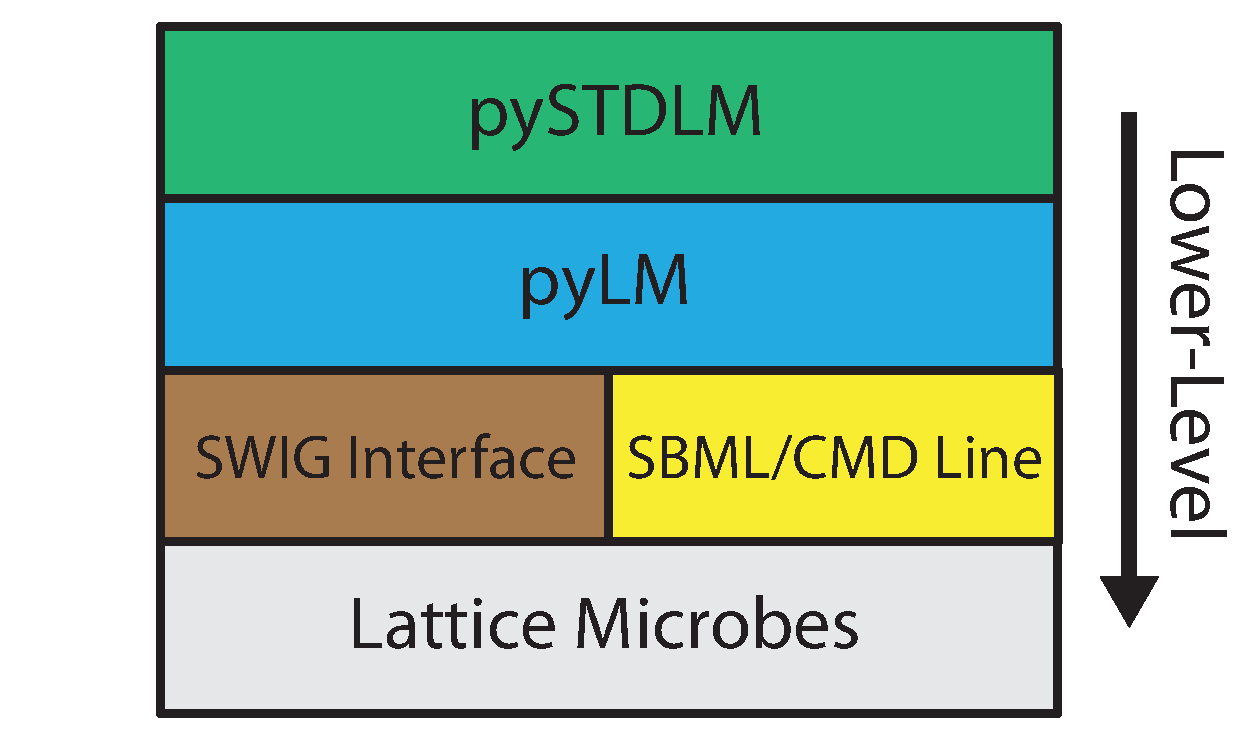
\includegraphics[width=0.7\textwidth]{Figures/Schematic.pdf}
  \caption{A schematic of the pyLM and the Lattice Microbes software.} \label{fig:pyschematic}
\end{figure}

The PSE is shown schematically in Figure \ref{fig:pyschematic}.  It sits on top of a SWIG interface that allows the C++ code to be accessible from the Python terminal.  Using pyLM allows the user to set up, run and post--process simulations all within a single script.  A general workflow for using LM is shown in Figure \ref{fig:workflow}.  For tutorials on using pyLM please see the ``Instruction Guide" and for in--depth description of all pyLM functionality please see the documentation ``Reference Guide" available on the website.

\begin{figure}[h!]
  \centering
      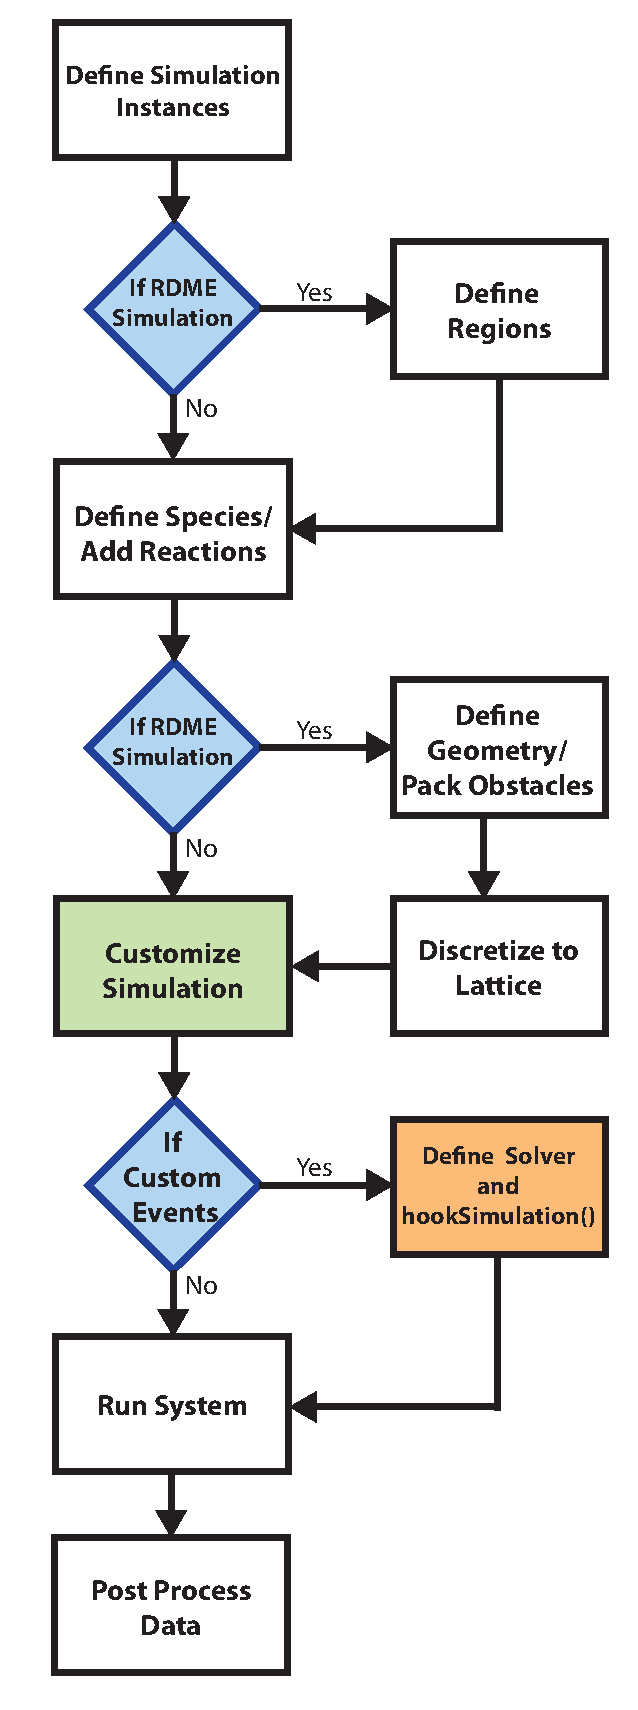
\includegraphics[width=0.5\textwidth]{Figures/Workflow.pdf}
  \caption{The workflow of the pyLM PSE.} \label{fig:workflow}
\end{figure}

\chapter{Capabilities}

%%%%%%%%%%%%%%%
% Section: SS %
%%%%%%%%%%%%%%%
\section{Stochastic Simulations}
Lattice Microbes can be used to simulate chemical master equations (CME):
\begin{equation*}
\frac{dP(\mathbf{x},t)}{dt}=\sum_{r}^{R} [-a_r({{\mathbf{x}}}) P({{\mathbf{x}}},t) + a_r({{\mathbf{x}}}_\nu-\mathbf{S_r}) P({{\mathbf{x}}}-\mathbf{S_r},t)]
\end{equation*}

\noindent and reaction-diffusion master equations (RDME):
\begin{align*}
\frac{dP(\mathbf{x},t)}{dt}=\sum_{\nu}^{V}\sum_{r}^{R} &[-a_r({{\mathbf{x}}}_\nu) P({{\mathbf{x}}}_\nu,t) + a_r({{\mathbf{x}}}_\nu-\mathbf{S_r}) P({{\mathbf{x}}}_\nu-\mathbf{S_r},t)]\\
+\sum_{\nu}^{V}\sum_{\xi}^{\pm\hat{i},\hat{j},\hat{k}}\sum_{\alpha}^{N} &[-d^{\alpha} x_{\nu}^{\alpha} P({{\mathbf{x}}},t) + d^{\alpha} (x_{\nu+\xi}^{\alpha}+1) P({{\mathbf{x}}}+1_{\nu+\xi}^{\alpha}-1_{\nu}^{\alpha},t)]
\end{align*}

\noindent using a variety of methods.  Both CME and RDME support a number of different reaction types including zeroth, first, second, and second order self reaction.  These reactions are of the form in Table \ref{tbl:rxnTypes}.  All rate constants input to Lattice Microbes should be the stochastic rate constant that has been scaled by the volume and Avogadro's number so that it is in units of \textbf{sec\textsuperscript{-1}}.  Use the table for the correct conversion factor.

\begin{sidewaystable}[htp]
\begin{center}
\begin{tabular}{|c|c|c|c|c|}
\hline
\textbf{Order} & \textbf{Form} & \textbf{Parameters} & \textbf{Macroscopic Units} & \textbf{Stochastic Rate Constant ($s^{-1}$)}\\
\hline\hline
0th  & $\emptyset \rightarrow \text{A}$   & $k$ & $Ms^{-1}$ & $k\cdot V \cdot N_A$\\
\hline
1st & $\text{A} \rightarrow \text{B}$ & $k$ & $s^{-1}$ & $k$ \\
\hline
2nd & $\text{A}+\text{B}\rightarrow \text{C}$ & $k$ & $M^{-1}s^{-1}$ & $\frac{k}{V\cdot N_A}$ \\
\hline
2nd (Self)\textsuperscript{*} & $2\text{A}\rightarrow\text{B}$ & $k$ & $M^{-1}s^{-1}$ & $\frac{k}{V\cdot N_A}$ \\
\hline
Michaelis-Menten\textsuperscript{$\dagger$} & $\text{E}+\text{S}\rightarrow\text{E}+\text{P}$ & $k_{cat}$, $K_{M}$ & $s^{-1}$, $M$ & $\frac{k_{cat}}{V\cdot N_A}$, $K_{M}V\cdot N_A$ \\ 
\hline
Competitive Michaelis-Menten\textsuperscript{$\dagger$} & $\text{E}+\text{I}+\text{S}\rightarrow\text{E}+\text{I}+\text{P}$ & $k_{cat}$, $K_{M}$, $K_{I}$ & $s^{-1}$, $M$, $M$ & $\frac{k_{cat}}{V\cdot N_A}$, $K_{M}V\cdot N_A$ , $K_{I}V\cdot N_A$\\ 
\hline
Uncompetitive Michaelis-Menten\textsuperscript{$\dagger$} & $\text{E}+\text{I}+\text{S}\rightarrow\text{E}+\text{I}+\text{P}$ & $k_{cat}$, $K_{M}$, $K_{I}$ & $s^{-1}$, $M$, $M$ & $\frac{k_{cat}}{V\cdot N_A}$, $K_{M}V\cdot N_A$ , $K_{I}V\cdot N_A$\\ 
\hline
Noncompetitive Michaelis-Menten\textsuperscript{$\dagger$} & $\text{E}+\text{I}+\text{S}\rightarrow\text{E}+\text{I}+\text{P}$ & $k_{cat}$, $K_{M}$, $K_{I}$ & $s^{-1}$, $M$, $M$ & $\frac{k_{cat}}{VN_A}$, $K_{M}V\cdot N_A$ , $K_{I}V\cdot N_A$\\ 
\hline
\end{tabular}
\end{center}
\caption{Reactions available to both CME and RDME.  Here, the stochastic rate constant should be computed from the macroscopic rate constant (perhaps from experiment) using the volume of the experiment, $V$, and Avogadro's number, $N_A$. \textsuperscript{*}Note that for a 2nd order self reaction, the rate of A disappearing is $2k$. \textsuperscript{$\dagger$}Michaelis-Menten type reactions are currently only supported in CME simulations, and only compute the propensity of forming the product using the steady-state assumption.} \label{tbl:rxnTypes}
\end{sidewaystable}%


In addition, the pyLM problem solving environment provides tools to setup, run and post-process stochastic simulations as well as integrate the stochastic techniques with other simulation methodologies (for example, see: \cite{Cole2014sso}).  The capabilities are outlined here.

\subsection{Well-Stirred Simulations}
CME simulations require species, reactions along with their rate constants, and initial specie counts to be specified.\\

A number of algorithms for sampling the CME are available with CPU and GPU implementations.  The Gillespie stochastic simulation algorithm (SSA) \cite{Gillespie1977ess} is the slowest but most straightforward.  The next-reaction (NR) and fluctuating next-reaction (FNR) \cite{Gibson2000ees} algorithms are also available and (may, depending on the count of particles) considerably speed up the simulation using variable time-stepping.  These techniques along with their capabilities can be found in Table \ref{tbl:cmeAlgorithms}. 


\begin{table}[htp]
\begin{center}
\begin{tabular}{|c|c|c|c|}
\hline
\textbf{Method} & \textbf{CPU} & \textbf{GPU} & \textbf{Solver Keyword} \\
\hline\hline
SSA & Y & Y & lm::cme::GillespieDSolver \\
\hline
NR & Y & Y & lm::cme::NextReactionSolver \\
\hline
FNR & Y & Y & lm::cme::FluctuatingNRSolver \\
\hline
\end{tabular}
\end{center}
\caption{CME sampling algorithms available in Lattice Microbes.  CPU and GPU columns indicate whether the algorithm is available (Y) or unavailable (N) for the particular compute device.  The Solver Keyword column indicates the string to pass to the ``lm" executable to perform that simulation.} \label{tbl:cmeAlgorithms}
\end{table}%





\subsection{Spatially-Resolved Simulations}
In addition to species, reactions along with their rate constants, and initial specie counts, RDME also requires the lattice spacing, spatial organization of objects (membrane, cytoplasm, etc.) and diffusion rates in and between these spatial objects to be specified.  \\

Two methods for solving the RDME are available in Lattice Microbes.  The first is the next subvolume (NS) method \cite{Elf2004ssb}, which is analogous to the next reaction method, of the CME.  The other is a constant timestep method called Multiparticle diffusion (MPD) developed to take advantage of the fine-grained parallelism afforded by the GPU \cite{Roberts2013lmh}.  In the latter case, the timestep is specified by the diffusion time:
\begin{equation*}
\tau=\frac{\lambda^2}{2\cdot n\cdot D}
\end{equation*}
\noindent where $\lambda$ is the lattice spacing, $n$ is the dimensionality (conventionally 2 or 3) and $D$ is the macroscopic diffusion constant. Both are GPU accelerated, while only one is available on the CPU as indicated in Table \ref{tbl:cmeAlgorithms}.

Additionally, a version of the MPD algorithm is available for computers with multiple-GPUs (called the MGPU-MPD solver) that can effectively and efficiently split the computation over the GPUs~\cite{Hallock2014sor}. 



\begin{table}[htp]
\begin{center}
\begin{tabular}{|c|c|c|c|}
\hline
\textbf{Method} & \textbf{CPU} & \textbf{GPU} & \textbf{Solver Keyword} \\
\hline\hline
NS & Y & Y & lm::rdme::NextSubvolumeSolver \\
\hline
MPD &N & Y & lm::rdme::MpdRdmeSolver \\
\hline
MGPU-MPD & N & Y & lm::rdme::MGPUMpdRdmeSolver \\
\hline
\end{tabular}
\end{center}
\caption{RDME sampling algorithms available in Lattice Microbes.  CPU and GPU columns indicate whether the algorithm is available (Y) or unavailable (N) for the particular compute device.  The Solver Keyword column indicates the string to pass to the ``lm" executable to perform that simulation.} \label{tbl:cmeAlgorithms}
\end{table}%


%%%%%%%%%%%%%%%%
% Section: PSE %
%%%%%%%%%%%%%%%%
\section{Problem Solving Environment}

pyLM and the included library of standard systems pySTDLM provide a problem solving environment for setting up, running and analyzing stochastic biological simulations \cite{Peterson2013aps}.  It contains functionality for specifying simulation setup including:

\begin{itemize}
\item Named species
\item Initial counts and distributions 
\item Reactions and rates
\item Spatial localization and definition
\item Diffusion properties
\item Obstacles
\item Define custom simulation flow
\end{itemize}

In addition, there are a number of pre- and post-processing functionalities including (but not limited to):

\begin{itemize}
\item Integration with Jupyter Notebook
\item Handles to data in the popular Numpy array representation
\item Plotting species averages/variances and individual time traces
\item Plotting Kymographs of spatial species distributions
\item Reaction network generation
\item Dynamic reaction network representations
\end{itemize}

The standard library (pySTDLM) also includes a number of cell shapes, colony layout routines, and previously published reaction systems.  Finally, pyLM provides functionality for accessing the underlying representation of the simulation data with time-based interrupts to allow users to modify or analyze the state of the simulation on-the-fly.  This last functionality allows there merger of different methodologies together.  For examples of how to use pyLM please refer to the ``Instruction Guide" and for full enumeration of functionality please see the ``Reference Manual" both of which are available online at \url{http://www.scs.illinois.edu/schulten/lm}. 




\chapter{Installation}

This chapter outlines the system and software requirements, and describes both methods of installing Lattice Microbes.  Installation of precompiled binaries is discussed in Section \ref{sec:binInstall}. Installation from source code is discussed in Section \ref{sec:srcInstall}.  Regardless of which of the two of these options is taken, pyLM requires additional installation instructions that are described in Section \ref{sec:pyInstall}.

%%%%%%%%%%%%%%%%%%
% Section: System Requirements %
%%%%%%%%%%%%%%%%%%
\section{System requirements} \label{sec:sysreq}

The Lattice Microbes software has been tested on Linux 2.6 and Mac OS X
10.8 and 10.9.  Although the software can be run entirely on a system's
CPU, Lattice Microbes was designed from the ground up to take advantage of
NVIDIA Fermi (compute 2.0) and later GPUs which allow for
orders-of-magnitude speedup over the CPU-only implementations.\\

%%%%%%%%%%%%%%%%%%
% Section: Software Requirements %
%%%%%%%%%%%%%%%%%%
\section{Software Requirements} \label{sec:softwarereq}

In order to take full advantage of the Lattice Microbes software, several external software packages should be installed on your system. While these lists appear daunting, the majority of the software have binary installers that simplify installation. The full enumeration of required packages:

\begin{itemize}[noitemsep]
\item Lattice Microbes v2.2 --- \url{http://www.scs.illinois.edu/schulten/lm/}
\item CUDA v5.5+ --- \url{http://developer.nvidia.com/cuda-downloads/}
\item Python v2.7 --- \url{http://www.python.org/download/}
\item HDF v1.8.8+ --- \url{http://www.hdfgroup.org/HDF5/release/obtain5.html}
\item Protocol Buffers \textbf{v2.4.1} --- \url{http://code.google.com/p/protobuf/downloads/}
\item SBML v5.9+ --- \url{http://sourceforge.net/projects/sbml/files/libsbml/}
\item h5py v2.2.1+ --- \url{http://code.google.com/p/h5py/downloads}
\item NumPy and SciPy --- \url{http://www.scipy.org/install.html}
\item iGraph 0.6.5+ --- \url{http://igraph.sourceforge.net/download.html}
\item pygexf v0.2.2+ --- \url{http://pythonhosted.org/pygexf/users.html}
\item lxml 3.2.4+ --- \url{https://pypi.python.org/pypi/lxml}
\item matplotlib v1.3.0+ --- \url{http://matplotlib.org/downloads.html}
\end{itemize}

Additional (highly recommended) optional packages:

\begin{itemize}[noitemsep]
\item VMD v1.9+ --- \url{http://www.ks.uiuc.edu/Research/vmd/}
\item Gephi v0.8.2+ --- \url{https://gephi.org/}
\item Cytoscape v3.0+ --- \url{http://www.cytoscape.org}
\item An MPI Library:
\begin{itemize}[noitemsep]
\item OpenMPI --- \url{http://www.open-mpi.org/software/ompi/v1.6/}, or
\item MPICH2 --- \url{http://www.mpich.org/downloads/}, or
\item MVAPICH2 --- \url{http://mvapich.cse.ohio-state.edu/download/}
 \end{itemize}
\end{itemize}

Requisite for GPU acceleration, users of NVIDIA Fermi or later GPUs should ensure that the CUDA 5.5+ drivers and libraries are installed and up to date.  \\

The popular molecular dynamics visualization and analysis software VMD can be used to view and animate output trajectories.  We believe that these capabilities are vital in understanding the details of how microscopic phenomena give rise to cell--scale behavior. For viewing of networks of interaction both statically and dynamically we recommend installing Gephi. Static networks can also be viewed with the popular Cytoscape graph visualizer. \\

Python scripts are used to set up and analyze realistic models of crowded cellular environments.  Users should ensure that Python is available on their system.  In addition, pyLM requires NumPy, SciPy, matplotlib, iGraph, h5py, lxml and pygexf for proper functioning. Most, if not all of these, are available as binaries, via a package manager (such as macports, apt, etc.) or via ``pip".\\

Some users may find it necessary to compile Lattice Microbes from source
code if, for example, they wish to create custom reaction rate equations
for their simulations, or will be installing Lattice Microbes on a compute
cluster, or a pre--compiled binary is not available for their machine.
The HDF5 and Protocol Buffers libraries and their development packages are required 
dependencies for source compilation.  See section \ref{source} for more
details.\\

The Systems Biology Markup Language, or SBML, is used to efficiently import complex reaction networks into LM kinetic/spatial models.  Users intending on compiling from source should download and install libSBML in order to ensure this functionality is available. \\

Finally, Lattice Microbes can be compiled with MPI in order to enable the distribution of replicates across many compute nodes on a cluster.  We recommend OpenMPI for clusters without Infiniband interconnects and MVAPICH for clusters with Infiniband.\\

Lattice Microbes is not a GUI program, it must be used from the command line. This enables it to efficiently run on \abr{HPC} clusters with minimal overhead. Consequently, all user interaction with the software, including installation, must be performed through the command line interface. In this chapter, commands to be executed from the command line are written as: ``\command{$\sim$/usr}{ls}'' which means to run the command ``\file{ls}'' from the directory ``\file{$\sim$/usr}''.

%%%%%%%%%%%%%%%%%%
% Section: Binary Installation %
%%%%%%%%%%%%%%%%%%
\section{Installing a precompiled binary} \label{sec:binInstall}

Available at the above url are several binaries precompiled for use either with or without GPU acceleration.  Users should select the binary appropriate for their system.\\

For the purposes of these instructions, it is assumed that the Lattice Microbes software will be installed into the directory \file{/home/<user>/usr}, also referred to as \file{$\sim$/usr}. If you wish to install the software elsewhere, please adjust the instructions accordingly.\\

Download the appropriate binary distribution to a temporary directory \file{/tmp}. Open a terminal and then change to the directory, unpack and copy the binary and libraries: \\

\command{$\sim$}{cd /tmp}\\
\command{/tmp}{tar zxvf lm-2.3\_<platform>.tgz}\\
\command{/tmp}{cp lm-2.3/bin/* $\sim$/usr/bin}\\
\command{/tmp}{mkdir -p $\sim$/usr/lib/lm}\\
\command{/tmp}{cp -r lm-2.3/lib/lm $\sim$/usr/lib/lm}\\
\command{/tmp}{cp -r lm-2.3/lib/python $\sim$/usr/lib/}\\

Copy the VMD plugin to the plugins/molefile directory of your VMD
installation: \\
\command{/tmp}{cp vmd/MACOSXX86/molfile/lmplugin.so /Applications/VMD\
1.9.1.app/\\
Contents/vmd/plugins/MACOSXX86/molfile} \hfill {\it (OS X)}\\

or:\\
\command{/tmp}{cp vmd/LINUXAMD64/molfile/lmplugin.so
/usr/local/lib/vmd/plugins/\\
LINUXAMD64/molfile} \hfill {\it (LINUX)}\\

\textbf{Note}: if you have installed the software into a non-global location, such as installing to \file{$\sim$/usr}, you will need to add the installation directory to you path. For example, you might add the following line to your \file{$\sim$/.bashrc} or \file{$\sim$/.bash\_profile} file:
{\small\begin{verbatim}
export PATH=$PATH:$HOME/usr/bin
\end{verbatim}}

Furthermore, if you have downloaded the CUDA version of Lattice Microbes, you must set the environment variable for the loader to find the CUDA libraries.  This can be done by adding the following line to your \file{$\sim$/.bashrc} or \file{$\sim$/.bash\_profile} file:\\

{\it (OS X)}
{\small\begin{verbatim}
export DYLD_LIBRARY_PATH=$DYLD_LIBRARY_PATH:/usr/local/cuda/lib
\end{verbatim}}

{\it (LINUX)} 
{\small\begin{verbatim}
export LD_LIBRARY_PATH=$LD_LIBRARY_PATH:/usr/local/cuda/lib
\end{verbatim}}

However, on Linux, this path may be slightly different, so if this command does not work, check your directory to make sure you have the right  PATH for the CUDA library.  If you are still unsure, check with your system administrator.\\

Finally, test the software installation:\\
 \command{/tmp}{lm --help}

If a help prompt is printed (enumerating the command line options) installation is likely correct. Otherwise, check that libraries are in the correct environmental paths.

%%%%%%%%%%%%%%%%%%
% Section: Source Installation %
%%%%%%%%%%%%%%%%%%
\section{Installing from source code} \label{sec:srcInstall}
\label{source}
As the computer architecture landscape becomes increasingly heterogeneous, many users may find that it is easiest to simply compile Lattice Microbes from source code on their own machine.  In order to accomplish this as painlessly as possible, this section is designed with the average user---not a software engineer---in mind.

\subsection{Satisfying external dependencies}

Although Lattice Microbes can be compiled and run without taking advantage of available GPU hardware, we believe that the real strength of the software is the orders-of-magnitude speedup gained through GPU acceleration.  In order to use Lattice Microbes to its fullest, you will first need to install the CUDA toolkit and drivers appropriate for your platform, if they are not installed already.  They can be found here:\\

\url{http://developer.nvidia.com/cuda-downloads}\\

The MacOSX installations are trivial---simply click through the installation wizards.  Linux installation can be somewhat more challenging, and will likely require you exit out of the GUI interface.  Help can be found here:\\

\url{http://docs.nvidia.com/cuda/cuda-getting-started-guide-for-linux/index.html}\\

Several other key features of the code also rely on external dependencies.  Python is required for programmatic setup of realistically crowded models of cells and analysis of simulation data.  The popular SBML file format can be used to import complex reaction networks. Both Python and libSBML should be installed prior to compiling the code, if they are not already.  MacOSX systems generally have Python pre-installed, but Linux users can find it via a package manager or download it here:\\

\url{http://www.python.org/download/}\\

The requisite SBML libraries can be found here:\\

\url{http://sourceforge.net/projects/sbml/files/libsbml/}\\

Again, installation on a Mac should be a breeze; installing libSBML for Linux should also be straightforward.  On Red Hat-based systems, the available .rpm package should be downloaded to a convienient location, such as \file{/home/<user>/usr}, and installed using rpm in a terminal window, for example:\\

\command{/home/<user>/usr}{rpm2cpio libSBML-5.6.0-Linux-x64.rpm  | cpio -idmv}\\

For Debian-derived distributions, the .deb package should be downloaded and installed using dpkg, e.g.:\\

\command{/home/<user>/usr}{sudo dpkg -i libSBML-5.6.0-Linux-x64.deb}\\

Although CUDA, Python, and libSBML are not {\it strictly} necessary, they impart functionalities crucial for studying large and complex biochemical systems under {\it in vivo} crowding conditions.  The Protocol Buffers and HDF5 libraries, on the other hand, are absolutely essential to compiling the code.  The protobuf library (version 2.4.1 only!!!) is used for serialization of messages across the transport layer. It is available from:\\

\url{http://code.google.com/p/protobuf/downloads/list}\\

This will need to be compiled from source.  Download the latest version to a convenient directory install:\\

\command{/home/<user>/usr}{tar zxvf protobuf-2.4.1.tar.gz}\\
\command{/home/<user>/usr}{cd protobuf-2.4.1}\\
\command{/home/<user>/usr/protobuf-2.4.1}{configure}\\
\command{/home/<user>/usr/protobuf-2.4.1}{make}\\
\command{/home/<user>/usr/protobuf-2.4.1}{sudo make install}\\

%The first of these commands queries several properties of your computer hardware and software, and sets up the make file.  The ``make" command compiles the source code, and the ``make install" command installs the compiled files to their proper locations.

The HDF5 library is used for reading models from and writing simulation data to HDF5 formatted files.  The HDF5 library is available from: \\

\url{http://www.hdfgroup.org/HDF5/release/obtain5.html}\\

Again, after downloading to a convenient directory extract the package, and move its contents to someplace that it is not likely to be moved, such as:\\
{\small\begin{verbatim}
/home/<user>/usr/hdf5-1.8.8-mac-x86_64-static/
\end{verbatim}}

Note the word ``static" in the directory above; static libraries, which end with extensions .a or .la for MacOS and LINUX, are compiled along with everything else into one monolithic executable binary.  Also available are shared or dynamic libraries, which end in .dylib or .so; these are not compiled into the executable binary, but rather remain separate and are linked to.  Whether you compile against static or dynamic libraries is up to you, but you will have to treat them differently when setting up your \texttt{local.mk} file, which will be described in Section \ref{staticDynamic}.\\

Finally, if you intend to compile with MPI for use on a compute cluster, you will need to acquire and install the requisite libraries.  There are several implementations of MPI available, and care should be taken in order to choose the right one for your cluster.

If one of the above packages is needed and is not already installed on your system, download a binary or source installation package and follow the installation instructions that accompany it. If you have problems, please contact your system administrator for assistance.

Note: if you install any external shared libraries into a non-global location, such as installing to \file{$\sim$/usr}, you will need to set an environment variable for the loader to find these libraries.
For example, you might add the following line to your \file{$\sim$/.bashrc} or \file{$\sim$/.bash\_profile} file:\\

{\it (OS X)}

\command{/home/<user>/usr}{export DYLD\_LIBRARY\_PATH=\$DYLD\_LIBRARY\_PATH:/usr/\\
local/cuda/lib}\\

{\it (LINUX)}

\command{/home/<user>/usr}{export LD\_LIBRARY\_PATH=\$LD\_LIBRARY\_PATH:/usr/\\
local/cuda/lib}\\

where /usr/local/cuda/lib is the path to a dynamic library you will be compiling against, in this case a CUDA library.  This will need to be done for all of the dynamic libraries you compile against.

\subsection{Unpack the source distribution}

For the purposes of these instructions, it is assumed that the Lattice Microbes software will be installed into the directory \file{/home/<user>/usr}, also referred to as \file{$\sim$/usr}. If you wish to install the software elsewhere, please adjust the instructions accordingly.\\

Download the source distribution from the URL above to the directory \file{$\sim$/usr/src}.  Then unpack the software:\\

\command{$\sim$}{cd $\sim$/usr/src}\\
\command{$\sim$/usr/src}{tar zxvf lm-2.3.tgz}\\
\command{$\sim$/usr/src}{cd lm-2.3}

\subsection{Configuring the build for your local environment}
\label{staticDynamic}
The Lattice Microbes source distribution ships with two default configuration files, one for Linux and one for Mac OS X. These files are located at:\\

\file{docs/config/local.mk.linux}\\
and\\
\file{docs/config/local.mk.osx}.\\

To begin, copy the file corresponding to your system to \file{local.mk}:\\

\command{$\sim$/usr/src/lm-2.3}{cp docs/config/local.mk.<platform> local.mk}\\

Edit the \file{local.mk} file to contain the correct options and file locations for your local environment. For example, if you installed the HDF5 and protobuf libraries into the \file{/home/<user>/usr} directory, you should set the PROTOBUF and HDF5 options as follows:

{\small\begin{verbatim}
HDF5_DIR := /home/<user>/usr
\end{verbatim}}
{\small\begin{verbatim}
PROTOBUF_DIR := /home/<user>/usr
\end{verbatim}}

Note: the HDF5 library actually has two dependencies of its own---SZIP and ZLIB---and the corresponding libraries are likely bundled with the software you downloaded.  This will work for linking dynamically against the libraries.

Each optional package has a section in the \file{local.mk} file that is initially disabled and begins with a line like:
{\small\begin{verbatim}
USE_XXXX := 0
\end{verbatim}}

To enable a specific package, set the flag corresponding to the package to 1 and set the options and locations appropriately. For example, if you are using Open MPI you might set the MPI options as follows:
{\small\begin{verbatim}
USE_MPI := 1
MPI_COMPILE_FLAGS = -DOMPI_SKIP_MPICXX=1 $(shell mpicc --showme:compile)
MPI_LINK_FLAGS = $(shell mpicc --showme:link)
\end{verbatim}}

For alternate MPI implementations you may need to experiment with the \file{mpicc} command to discover the correct settings or look at the example configuration files included with the Lattice Microbes source distribution.\\

If you are using Python 2.7 you might set the Python options as follows:
{\small\begin{verbatim}
USE_PYTHON := 1
PYTHON_SWIG := /usr/bin/swig
PYTHON_INCLUDE_DIR := `python-config --includes`
PYTHON_LIB := `python-config --libs`
\end{verbatim}}

If you are using CUDA with a capable device you might set the CUDA options as follows:
{\small\begin{verbatim}
USE_CUDA := 1
CUDA_DIR := /usr/local/cuda
\end{verbatim}}

The location of your CUDA\_DIR will depend on your installation of Cuda. ou may also need to change the CUDA\_ARCH variable to match your GPU version. You can determine your GPU's compute capability you need to enable by visiting \url{https://developer.nvidia.com/cuda-gpus}.

If you want to build Lattice Microbes with support for importing SBML files (and have libSBML installed to \file{/home/<user>/usr}) you might set the SBML options as follows:
{\small\begin{verbatim}
USE_SBML := 1
SBML_DIR := /home/<user>/usr
\end{verbatim}}

{\it (OS X)} If you want to build the VMD plugin and have VMD installed to the Applications folder you might set the VMD options to:
{\small\begin{verbatim}
USE_VMD := 1
VMD_DIR := "/Applications/VMD\ 1.9.1.app/Contents/vmd"
\end{verbatim}}

{\it (LINUX)} If you want to build the VMD plugin and have VMD installed to \file{/usr/local} you might set the VMD options to:
{\small\begin{verbatim}
USE_VMD := 1
VMD_DIR := /usr/local/lib/vmd
\end{verbatim}}

Finally, you should set the installation location and build name for the Lattice Microbes software at the top of the \file{local.mk} file:
{\small\begin{verbatim}
BUILD_DIR := Build-osx
INSTALL_PREFIX := /home/<user>/usr
\end{verbatim}}

\subsubsection{Additional Compile Time Features}

There are additional compile time flags that can be enabled to allow for
nonstandard features in Lattice Microbes.  They can be enabled by adding
the option to both CCFLAGS and CUDA\_FLAGS defined in your \file{local.mk}.
These are:

\begin{description}
\item[-DGLOBAL\_S\_MATRIX] \hfill \\ Enable this flag if your stoichiometry matrix is large.  By default the S matrix is stored in GPU constant memory,  and therefore the number of species times the number of reactions must be less than 4096 (16KB).  By enabling this feature, the maximum size of the S matrix is increased to 262144 (1MB) allowing for up to 1536 reactions with 256 species.
\item[-DLATTICE\_MAX\_OCCUPANCY=16] \hfill \\ Enabling this flag doubles the maximum particles per site from 8 to 16, doubling the memory cost and potentially slowing the simulation speed.  \textbf{WARNING: There is no support for 8/16 particle lattice interoperability.  Files created by code with a specific occupancy should only be read and written by binaries built with the same value.}
\item[-DFREAKYFAST] \hfill \\ For MPD-RDME, use the reaction kernel with pre-computed reaction propensities~\cite{Hallock2016irk}.  This accelerates simulations with large numbers of reactions.
\end{description} 

\subsubsection{Enabling Profiling}

Profiling of Lattice Microbes is available via the NVTX API, and profiling
information can be captured with the Nvidia command-line profiler (nvprof)
or via the Visual Profiler (nvcc).  To enable, add the following feature
flags in to \file{local.mk}. 

USE\_PROF := 1 \\
USE\_PROF\_NVTX := 1

\subsection{Build and install the software}

Now that the build is configured, build and install the source code:\\

\command{$\sim$/usr/src/lm-2.3}{make LOCALMK=local.mk}\\
\command{$\sim$/usr/src/lm-2.3}{sudo make install}\\

Note: if you have installed the software into a non-global location, such as installing to \file{$\sim$/usr}, you will need to add the installation directory to you path. For example, you might add the following line to your \file{$\sim$/.bashrc} file:
{\small\begin{verbatim}
export PATH=$PATH:$HOME/usr/bin
\end{verbatim}}

Finally, test the software installation:\\

 \command{$\sim$/usr/src/lm-2.3}{lm --help}\\
 
If no errors occur, the software is installed correctly.  If you get errors about a missing library, you will likely have to add their paths to the library path environment variable.  


%%%%%%%%%%%
%Section: pyLMInstall%
%%%%%%%%%%%
\section{pyLM Installation} \label{sec:pyInstall}

pyLM comes with both the source and the binary distribution of Lattice Microbes.  Configuring pyLM to work requires installing external software and setting environment paths to the correct locations. \\

One the Lattice Microbes installation is complete, the paths that Python looks for code in must be updated.  Add the paths to your  \file{$\sim$/.bashrc} or \file{$\sim$/.bash\_profile}:

\begin{verbatim}
export PYTHONPATH=/home/<user>/usr/lib/lm:$PYTHONPATH
export PYTHONPATH=/home/<user>/usr/lib/python:$PYTHONPATH
\end{verbatim}

\subsection{External Libraries}
The instructions in this section may only be applicable for the particular version of the libraries that are listed.  If the installation fails, please see the documentation on the website or in the tar file.  Most of these can be installed via a package manager or via ``pip".

\subsubsection{Installing h5py}

Once downloaded, h5py can be installed with the following set of commands:\\

\command{/tmp}{tar -xvf h5py-2.2.0.tar.gz} \\
\command{/tmp}{cd h5py-2.2.0} \\
\command{/tmp/h5py-2.2.0}{python setup.py build --hdf5=/home\\/<user>/usr/hdf5-1.8.8-mac-x86\_64-static/lib} \\
\command{/tmp/h5py-2.2.0}{python setup.py test} \\
\command{/tmp/h5py-2.2.0}{sudo python setup.py install} \\

Alternatively, this can be installed via pip:\\

\command{/tmp}{pip install h5py}\\

\subsubsection{Installing NumPy}

NumPy can be installed on almost any system from binary.

\subsubsection{Installing SciPy}

SciPy can be installed on almost any system from binary.

\subsubsection{Installing iGraph}

iGraph can be installed for Mac from binary.  

\noindent For Linux machines, you must first install the C library: \\

\command{/tmp}{tar -xvf igraph-0.6.5.tar.gz} \\
\command{/tmp}{cd igraph-0.6.5} \\
\command{/tmp/igraph-0.6.5}{./configure} \\
\command{/tmp/igraph-0.6.5}{make} \\
\command{/tmp/igraph-0.6.5}{sudo make install} \\


\noindent Then the following commands may be used to build the python interface: \\

\command{/tmp}{tar -xvf python-igraph-0.6.5.tar.gz} \\
\command{/tmp}{cd python-igraph-0.6.5} \\
\command{/tmp/python-igraph-0.6.5}{python setup.py build} \\
\command{/tmp/python-igraph-0.6.5}{sudo python setup.py install} \\

Alternatively, this can be installed via pip:\\

\command{/tmp}{pip install python-igraph}\\

\subsubsection{Installing pygexf}

First, you must install lxml: \\

\command{/tmp}{tar -xvf lxml-3.2.4.tar.gz} \\
\command{/tmp}{cd lxml-3.2.4} \\
\command{/tmp/lxml-3.2.4}{python setup.py build} \\
\command{/tmp/lxml-3.2.4}{sudo python setup.py install} \\

Alternatively, this can be installed via pip:\\

\command{/tmp}{pip install lxml}\\

Finally, you can install pygexf: \\

\command{/tmp}{unzip pygexf-master.zip} \\
\command{/tmp}{cd pygexf-master} \\
\command{/tmp/lxml-3.2.4}{sudo easy\_install pygexf} 

\subsection{Testing}

Several test input files are included in the pyLM distribution.  To test that pyLM and Lattice Microbes are installed correctly, go to the ``src/python/Examples" directory in the source directory and execute the command: \\

\command{/tmp}{python example-bimol.py  -o cmebimol.lm} \\

\noindent If no errors are reported, these programs are installed correctly.  Next, a test of the correct installation of the other libraries should be performed.  Execute the following command in the same directory: \\

\command{/tmp/}{python example-bimol-pp.py -o cmebimolpp.lm} \\

\noindent If all goes well, two plots will be made in the directory named ``BimolSpeciesTrace.png" and ``BimolSpeciesFit.png".  In addition, a graph file named ``BimolGraph.gml" will be made in that directory which can be opened with popular network viewing software such as Gephi (\url{https://gephi.org}) or Cytoscape (\url{http://www.cytoscape.org}). Representative examples of each of these file can be seen in Figures \ref{fig:bst}, \ref{fig:bsf} and \ref{fig:graph}.


\begin{figure}[h!]
  \centering
      \includegraphics[width=0.75\textwidth]{Figures/BimolSpeciesTrace.png}
  \caption{Average (top) and Variance (bottom) of  the three species over 50 replicates for the reversible bimolecular reaction.} \label{fig:bst}
\end{figure}

\begin{figure}[h!]
  \centering
      \includegraphics[width=0.75\textwidth]{Figures/BimolSpeciesFit.png}
  \caption{The same figure as before, except with fits to the rates performed in Python.} \label{fig:bsf}
\end{figure}

\begin{figure}[h!]
  \centering
      \includegraphics[width=0.75\textwidth]{Figures/RxnGraph.pdf}
  \caption{The graph of the simple bimolecular reaction.  Nodes in cyan are reacting species and red are reactions.  Direction of the arrows indicate flow of reactants.} \label{fig:graph}
\end{figure}


%%%%%%%%%%%
%Section: Difficulty%
%%%%%%%%%%%
\section{In case of difficulty}
If you experience problems when building the software, email the Lattice Microbes User List:\\ \url{latticemicrobes-users@lists.illinois.edu}.

Also, consider joining the Lattice Microbes User List by visiting: \\ \url{https://lists.illinois.edu/lists/info/latticemicrobes-users}



%%%%%%%%%%%%%%%%%%%%%
% Section: Examples %
%%%%%%%%%%%%%%%%%%%%%
\chapter{Examples Simulation Specifications}
Many examples demonstrating features of pyLM exist both on the website (\url{http://www.scs.illinois.edu/schulten/lm/download/lm22/ExampleFiles.tgz}) and in the source code (\texttt{src/python/Examples}).  Each demonstrates several different features of pyLM, and it is suggested that you read and work through all of the examples before starting to use pyLM for your project.  It is recommended that you work through the problems in the order shown, as functionality documented in an earlier file is not described again in later files.

Various functionality is demonstrated in the examples, including:

\begin{itemize}
\item CME
\begin{enumerate}
\item example-bimol.py -- Demonstrates process of defining molecular species, reactions  and initial conditions in a CME simulation
\item example-bimolConc.py -- Same as example-bimol.py using concentrations instead of particle numbers
\item example-bimol-pp.py -- Demonstrates the general trends for writing post-processing code for a CME simulation
\item example-rnaprotein.py -- An example of constitutive gene expression
\item example-LotkaVolterra.py -- An example of the well known Lotka-Volterra problem (predator-prey) simulated with stochasticity
\item example-stochasticResonator.py -- An example of a stochastic resonator problem with CME
\item example-lac2state.py -- This file demonstrates a more complex reaction scheme
\end{enumerate}

\item RDME
\begin{enumerate}
\item example-MichaelisMenten.py -- This demonstrates how to define a simulation domain in a 3D RDME simulation and defines an enzyme/substrate reaction system to be simulated in the domain
\item example-minde.py -- A demonstration of the popular Min system of {\it E. coli} showing how to construct default cell shapes, customize diffusion coefficients in regions and diffusion coefficients between regions
\item example-restart.py -- This demonstrates how to restart an RDME simulation, however it is a hack as of now
\end{enumerate}

\item Advanced Setup
\begin{enumerate}
\item example-shapes.py -- An example showing how to define complex objects such as boxes, spheres, tori, ellipses and intersections, unions and differences of the various objects
\item example-tightPackedCellArray.py -- This example shows a pySTDLM feature that packs a cell shape into a tight regular grid spanning the whole RDME domain
\item example-extendrdme.py -- This example shows how to extend the basic RDME solver with a hook that is run on every lattice write, allowing the user to modify the simulation based on the simulation state
\end{enumerate}
\end{itemize}

\input{Text/License}


%%%%%%%%%
% References %
%%%%%%%%%
\newpage
\addcontentsline{toc}{chapter}{Bibliography}
\bibliographystyle{Bibliography/inorder}
\bibliography{Bibliography/references,Bibliography/zlsgroup-2016}


\end{document}
